\documentclass[titlepage, twocolumn, a4paper, 12pt, swedish]{article}
\usepackage[swedish]{babel}
\usepackage[utf8]{inputenc}
\usepackage{verbatim}
\usepackage{fancyhdr}
\usepackage{graphicx}
\usepackage{parskip}
\usepackage{enumerate}
\usepackage{varioref}

% Column spacing
\setlength{\columnsep}{10mm}

% SourceCode
\usepackage{listings}
\usepackage{color}

% Include pdf with multiple pages ex \includepdf[pages=-, nup=2x2]{filename.pdf}
\usepackage[final]{pdfpages}
% Place figures where they should be
\usepackage{float}

% SourceCode
\definecolor{keywordcolor}{rgb}{0.5,0,0.75}
\lstset{
  inputencoding=utf8,
  language=Java,
  extendedchars=true,
  basicstyle=\scriptsize\ttfamily,
  stringstyle=\color{blue},
  commentstyle=\color{red},
  numbers=left,
  firstnumber=auto,
  numberblanklines=true,
  stepnumber=1,
  showstringspaces=false,
  keywordstyle=\color{keywordcolor}
  % identifierstyle=\color{identifiercolor}
}

% Float for text
\floatstyle{ruled}
\newfloat{kod}{H}{lop}
\floatname{kod}{Kodsnutt}

% vars
\def\title{Genetisk animation; rörelsemönster i 2D mha neuralt nät och genetisk algoritm}
\def\preTitle{Projekt}
\def\kurs{Emergenta system, 5DV017}
\def\namn{Andreas Jakobsson}
\def\mail{dit06ajs@cs.umu.se}

\def\namnTva{Anton Johansson}
\def\mailTva{dit06ajn@cs.umu.se}

\def\namnTre{Erik Rönnberg}
\def\mailTre{dit06erg@cs.umu.se}

\def\namnFyra{Ludvig Widman}
\def\mailFyra{dit06lwn@cs.umu.se}

\def\namnFem{Ragnar Asplund}
\def\mailFem{dit04rad@cs.umu.se}

\def\pathtocode{http://github.com/blastura/genetic-reanimation/tree/master}

\def\handledareEtt{Jonny Pettersson, jonny@cs.umu.se}
\def\handledareTva{Anders Broberg, bopspe@cs.umu.se}

\def\inst{datavetenskap}
\def\dokumentTyp{Projektrapport}

\begin{document}
\begin{titlepage}
  \thispagestyle{empty}
  \begin{small}
    \begin{tabular}{@{}p{\textwidth}@{}}
      UMEÅ UNIVERSITET \hfill \today \\
      Institutionen för \inst \\
      \dokumentTyp \\
    \end{tabular}
  \end{small}
  \vspace{10mm}
  \begin{center}
    \LARGE{\preTitle} \\
    \huge{\textbf{\kurs}} \\
    \vspace{10mm}
    \LARGE{\title} \\
    \vspace{15mm}
    \begin{large}
      \namn, \mail \\
      \namnTva, \mailTva\\
      \namnTre, \mailTre\\
      \namnFyra, \mailFyra\\
      \namnFem, \mailFem\\
      \texttt{\pathtocode}
    \end{large}
    \vfill
    \large{\textbf{Handledare}}\\
    \mbox{\large{\handledareEtt}}
    \mbox{\large{\handledareTva}}
  \end{center}
\end{titlepage}

\newpage
\mbox{}
\vspace{70mm}
\begin{center}
% Dedication goes here
\end{center}
\thispagestyle{empty}
\newpage

\pagestyle{fancy}
\rhead{\today}
\lhead{\footnotesize{\mail, \mailTva\\\mailTre, \mailFyra, \mailFem}}
\chead{}
\lfoot{}
\cfoot{}
\rfoot{}

\begin{abstract}
% TODO: Sammanfattning/abstract
Genetic algorithms have been used to evolve movement of virtual creatures in a number of occasions. This Report describes a simple simulation for evolving movements of a worm over time and generations. A simplified and modified 2D version of Karl Sims work with Evolving Virtual Creatures is created. Creatures are created with a random genotype, the creatures movements are simulated and patterns arise from a Hopfield neural network. The genotype is simply all the weights of the neural network which evolve over generations from a Genetic Algorithm. The fitness for each creature is determined by how far they are able to move within a set number of steps. A large number of tests are made and a rolling or a combination of rolling and jumping movement seems to be the most effective pattern for forward movement.
\end{abstract}
 
\cleardoublepage
\newpage
\onecolumn
\tableofcontents
\cleardoublepage
\twocolumn
\cfoot{\thepage}
\pagenumbering{arabic}


\section{Introduktion}
% Introduktion till ämnet, inklusive översikt av tidigare studier
% \cite{flake}

I detta projekt har vi undersökt möjligheten att utveckla rörelsemönster för en enkel varelse med hjälp av genetiska algoritmer. Varelsen har ett neuralt nät som ”hjärna” och har formen av en ledad ”mask”.

\subsection{Karl Sims}
Karl Sims utforskar i Evolving Virtual Creatures \cite{sims} både hur varelsers form och deras beteenden kan utvecklas med hjälp av genetiska algoritmer (GA). Varelserna har sensorer och effektorer som är kopplade till in- och utnoder i ett neuralt nät. 

I sina försök använder Sims en GA för att optimera både struktur och vikter i det neurala nätet. Det nät han använder har i varje nod en av många matematiska funktioner; exempelvis sinus, summa, produkt, max, osv. Sims lät sina försök köra mellan 50 och 100 generationer och optimerade mot olika typer av beteenden som ex gång, simmande och hoppande rörelser. 

\subsection{Hugo de Garis}
Hugo de Garis forskning i \textit{Genetic Programming: Evolutionary Approaches to Multistrategy Learning} \cite{garis} inriktar sig i störst utsträckning mot utveckling av hårdvara med hjälp av genetiska algoritmer. Han beskriver metoder som shaping (att i olika steg ändra definitionen för fitness) och talar om "utvecklingsbara system" med de avseendet att vissa system inte går att ge önskvärt beteende med hjälp av genetiska algoritmer. Han nämner att de inte finns något sätt att definitivt avgöra vilka system som är utvecklingsbara med fasta kriterier.

Garis har utvecklat en simulerad ödla som han kallar \textit{LIZZY} \cite{garis}. Den virtuella ödlan \textit{LIZZY} känner sin omvärld med två antenner och tar därigenom emot karaktäristiska signaler från tre sorters kreatur i dess omgivning; Mate, Prey och Predator. Med hjälp av ett neuralt nät och en genetisk algoritm lär sig sedan \textit{LIZZY} att söka upp Prey och Mate, där vidta passande åtgärder, och att fly undan Predators.

\subsection{Syfte}
Inledningsvis valde vi ämnet rörelsemönster i 2D mha Genetiska algoritmer. Vi ville utforska ämnet GA lite djupare och tyckte Sims försök var en bra utgångspunkt. 

I detta arbete har vi försökt återskapa en förenklad variant på Sims arbete. Istället för tre dimensioner använder vi bara två. Dessutom använder vi bara en fix varelse och en enklare hjärna. 

Vi vill se om denna förenklade modell kommer hitta fungerande rörelsemönster. Hur effektiv den är på detta och hur intressant resultatet blir kommer också studeras. 
%Vilka faktorer är viktiga/har stor påverkan på resultatet vid simulering av rörelsemönster.

% Frågeställning fylls i här typ

%Kan en GA hitta ett naturligt rörelsemönster för ett enkelt 2d-djur? 
%Hur effektiva är GAs på att hitta fungerande rörelsemönster? 
%Kan vi upprepa Browns, Nicolas Lassabe eller Karl Sims simuleringar i en 
%2D-miljö? åäö.


\section{Metodbeskrivning}
% Metodbeskrivning. Ska beskrivas så utförligt att läsaren ska kunna
% reproducera ert arbete
% Systemet består av tre stora delar. Den genetiska algoritmen (GA), Hjärnan och Fysiksimuleringen. 
Vi har utvecklat ett system som utvecklar kroppars rörelsemönster med hjälp av en genetisk algoritm. Kroppen simuleras i en fysikmotor och rörelsen bestäms av ett neuralt nät där indata kommer från simuleringsvärlden och utdata ansätts till varelsens effektorer. Fitnessfunktionen beräknas enligt längden varelsen har tagit sig på sin förinställda livslängd.

% Alltid en början av en början...

\subsection{Varelser}
I följande stycke presenteras en översikt av hur en varelse är uppbyggd och hur den reagerar/agerar på omvärlden.

\subsubsection{Uppbyggnad av varelse}\label{sec:uppbyggnadVarelse}
Varelsen består av en mask med 4 leder och 5 kroppsdelar, se \ref{fig:creature.pdf}. Varje led kan röra sig 180 grader. Varje kroppsdel har en sensor som ger \textit{hjärnan} indata om dess y-position i förhållande till delen utmed. Att en maskliknande varelse har valts beror på att kroppen är relativ enkel i sin sammansättning och komplexiteten sjunker således. Kroppsdelarnas vikt, ledernas typ och ledernas rörelsefrihet har valts efter eget tycke då varelsen ses som ett inledande exempel på hur systemet kan fungera. Valet av indata för varelsen grundas i en önskan om ledernas vetskap om varandra. Källkod för den implementerade varelsen finns i bilaga \ref{app:WormCreature}.

\begin{figure}
  \begin{center}
    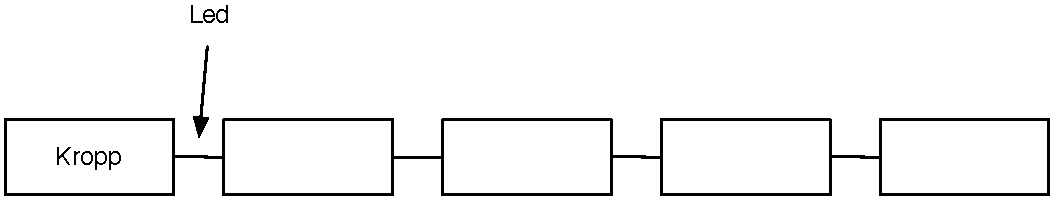
\includegraphics[width=78mm]{images/creature.pdf}
    \caption{Representation av varelse}
    \label{fig:creature.pdf}
  \end{center}
\end{figure}

\subsubsection{Sensorer}
Varelsens sensordata räknas ut som differensen mellan kroppdelarnas y-position. Antalet sensorer/indata blir ett mindre än antalet kroppsdelar då de räknas ut mellan intilliggande kroppsdelar. 

\subsubsection{Effektorer}
% Joints
Varelsens effektorer utgörs i implementationen av en viss typ av leder som krafter kan appliceras på. Efter att varelsens \textit{hjärna} har bearbetat indata så hämtas utdata som nu kommer att vara mellan -1 och 1. Denna utdata multiplicaras med $\pi$ för att få en vinkel mellan $-\pi$ och $\pi$, det resulterade värdet låtes påverka leden, som i sin tur påverkar de två kroppar leden är fäst vid.

\subsubsection{Neuralt nät}
% Neuroner
Varelsens hjärna består av ett neuralt nät som styr dess beteende. Det neurala nätet är vagt implementerat enligt Hopfields modell för neurala nät, se kapitel 13 i boken \textit{Neural networks: a systematic introduction}, se \cite{raul}. Varje nod i det neurala nätet har bågar till och från alla andra noder. Varje båge har en vikt.

För att mata nätet med indata tas värden emot och körs genom en sigmoid funktion $1/\frac{1}{1 + e^{-x}}$. Denna funktion är modifierad för att ge resultat mellan -1 och 1. Sigmoidfunktionen är uppritad i figur \vref{fig:sigmoid}. Javakod för sigmoid-funktionen som används visas i kodsnutt \ref{kod:sigmoid}. Vid varje simuleringssteg i hjärnan beräknas ett värde i varje nod. Värdet beräknas som en summa av värdet från varje båge gånger dess vikt. På denna summa appliceras sedan sigmoidfunktionen så värdet hamnar mellan -1 och 1.

\begin{figure}
    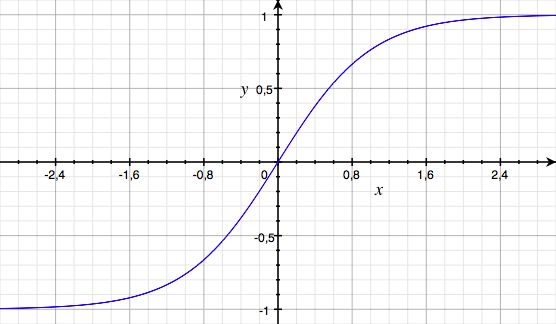
\includegraphics[width=78mm]{images/sigmoid.jpg}
    \caption{Plot av sigmoidfunktionen}
    \label{fig:sigmoid}
\end{figure}

Det görs ingen skillnad bland noderna i nätetet med avseende på vilka som tar emot och ger ifrån sig in- och utdata. Det neuralal nätet tar emot indata i from av en vektor, positionen värdena har i vektorn avgör vilken nod i nätet som kommer att ta emot datan. Samma position i vektorn kommer alltid att motsvara samma nod i det neurala nätet. Utdata fås ur det neurala nätet genom att alla noders värden returneras som en vektor. Behövs inte all utdata är det upp till den anropande metod att välja ut vilka nod-värden som ska användas.

\begin{kod}
\begin{footnotesize}
\begin{verbatim}
2 / (1 + Math.pow(Math.E, (-2 * x))) - 1
\end{verbatim}
\end{footnotesize}
\caption{Sigmoid (java)}\label{kod:sigmoid}
\end{kod}

\begin{figure}[H]
  \begin{center}
    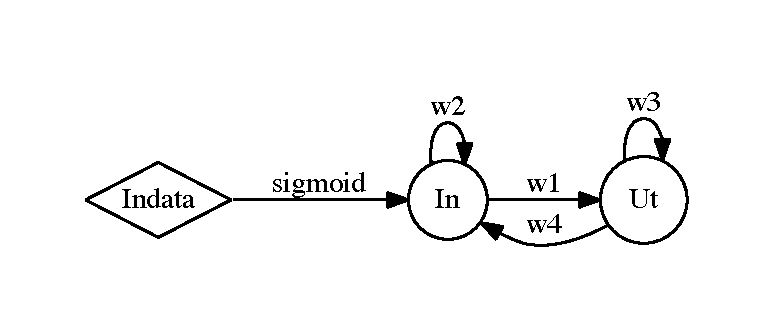
\includegraphics[width=78mm]{images/neuralnet.pdf}
    \caption{Neuralt nätverk med två noder}
    \label{fig:neuralnet.pdf}
  \end{center}
\end{figure}

%tänkte mig lista klasser här så det blir en systemöversikt? 
%\begin{enumerate}[(a)]
%\item ...  ...
%\item hej
%\end{enumerate}

Källkoden för implementationen av det neurala nätet finns i bilaga \ref{app:HopfieldNeuralNet}.

\subsection{Simulering}
Fysiksimuleringen använder biblioteket \textit{phys2d} \cite{phys2d} för själva fysiken. Detta bibliotek är skrivet av Kevin Glass och är en Java-variant av Erin Catto's plattform \textit{box2d} \cite{box2d}. Denna platform valdes på grund av att den bygger på Java och gruppen besitter kompetens inom språket. I simuleringen har ett markplan skapats och på detta en varelse. En vägg skapades även till vänster om masken för att förhindra att den försvinner bakåt ur fönstret.

\subsection{Genetisk algoritm}
För selektion används en variant på tournament selection. Först skapas en ny tom population, den bästa individen från föregående generation kopieras sedan in i den nya populationen. Två grupper om tre individer väljs sedan slumpmässigt och de med högst fitness ur respektive grupp korsas så två nya varelser med en blandning av deras genotyp skapas. Detta upprepas tills en bestämd del av en ny population har skapats, detta bestäms av mutation-rate i programmet. Därefter väljs fler grupper av tre där de bästa direkt går till den nya populationen oförändrade tills den nya populationen har samma storlek som den gamla. Varje individ utom den första med högst fitness i den nya populationen muterar sedan varje del av sin genotyp med en viss sannolikhet. Den nya populationen ersätter därefter den gamla. 

Genotypen i varelsen kodar för vikter i det neurala nät som utgör dess hjärna. För att evaluera fitness för varje individ skapas ett nät med de vikter genotypen anger, detta får sedan under en begränsad tid styra en fast kropp i en fysiksimulering. Fitness beräknas på hur långt kroppen lyckats röra sig.

\begin{enumerate}
\item skapa en ny tom population
\item kopiera över den individ med högst fitness från föregående generation till den nya populationen
\item upprepa till den bestämda andel crossover till nya generationen är utförd
\begin{enumerate}
\item välj ut två grupper om tre individer
\item utför crossover på den individ med högst fitness från respektive grupp och lägg över deras barn till den nya populationen
\end{enumerate}
\item upprepa till den nya populationen har samma storlek som den föregående generationen
\begin{enumerate}
\item välj grupp om tre individer
\item kopiera över den individ med högst fitness från de tre
\end{enumerate}
\item mutera varje individ utom den första med högst fitness
\end{enumerate}

Källkoden till den genetiska algoritmen som används finns i bilaga \ref{app:GeneticAlgoritm}.

\section{Resultat}

\subsection{Rörelsemönster}
För att undersöka vilka rörelsemönster som får hög fitness har vi gjort ett stort antal testkörningar och spelat in den bästa varelsen i varje generation. Därefter har typiska rörelser med bra fitness valts ut och presenterats i form av bilder. Det vanligaste rörelsemönstret är att masken rullar fram, det visas i figur \vref{fig:r1}. Ett annat rörelsemönster, hopp-rullande, som hade något högre fitness visas i figur \vref{fig:r2}.


% Resultat innehållande sammanställning/analys av tester
\begin{figure}
    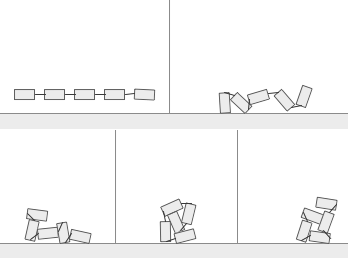
\includegraphics[width=78mm]{images/mask1_gs.png}
    \caption{Ett typiskt rörelsemönster där masken rullar fram.}
    \label{fig:r1}
\end{figure}

\begin{figure}
    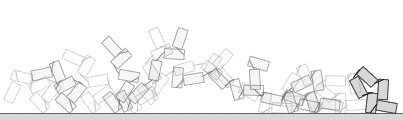
\includegraphics[width=78mm]{images/maskninja.png}
    \caption{Hopp-rullande rörelse. Dessa rörelser är ofta lite effektivare än bara rullande.}
    \label{fig:r2}
\end{figure}

\subsection{Fitness}
För att undersöka hur fitness utvecklas har vi har testat att köra simuleringen ett flertal gånger och låta den köra i 15-20 generationer. Därefter plotat medel max och min för fitness i varje generation. Detta syns i figuerna \vref{fig:d1}, \vref{fig:d2} och \vref{fig:d3}. De olika figurerna skiljer sig ganska mycket, men visar ändå karakteristiska egenskaper vi sett i de flesta av våra körningar så som att max-fitness ökar etappvis. Oftast stiger medelvärdet sakta över tiden.

\begin{figure}
    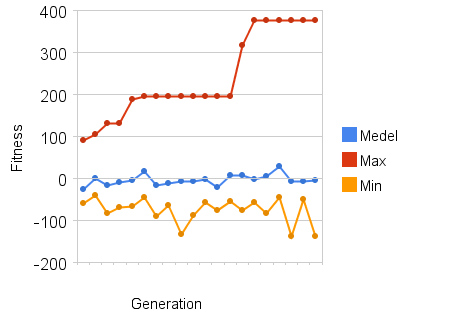
\includegraphics[width=78mm]{images/diagram4.png}
    \caption{Fitnessens utveckling över 20 generationer.}
    \label{fig:d1}
\end{figure}

\begin{figure}
    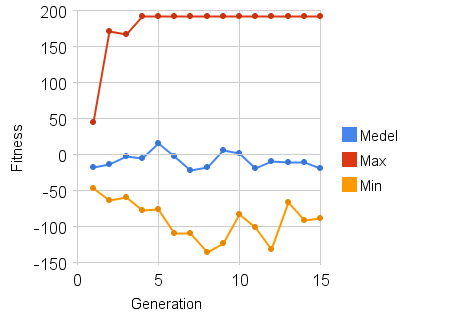
\includegraphics[width=78mm]{images/diagram3.png}
    \caption{Fitnessens utveckling över 15 generationer.}
    \label{fig:d2}
\end{figure}

\begin{figure}
    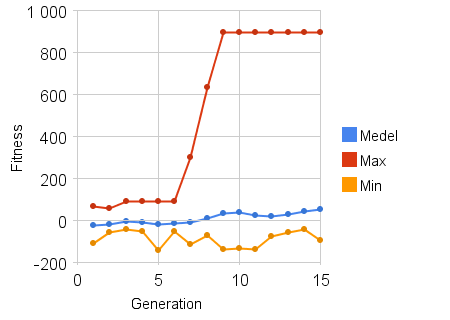
\includegraphics[width=78mm]{images/diagram_m01c08_2.png}
    \caption{Fitnessens utveckling över 15 generationer.}
    \label{fig:d3}
\end{figure}

\section{Diskussion}
Ett flertal olika rörelsemönster hittades av vår algoritm. Många av dem var bara spasmiska eller icke-cykliska (dvs varelsen fastnar och stannar). Några rörelsemönster fungerade väl och förflyttade masken effektivt frammåt. 

Man kan konstatera att vår enkla modell fungerar för att hitta rörelsemönster, men resultatet blir inte lika intressant som för Sims. Detta kan dock delvis förklaras med att en mask inte kan röra sig på så många olika sätt öht.

Det rörelsemönster som gett mest framgång i våra studier är ett rullande eller rull-hoppande beteende. En förklaring till att detta mönster är vanligt i våra simuleringar, men inte i verkligheten kan vara att 2D-maskar inte kan tippa i sidled. Det är även tänkbart att våra simulerade maskar är starkare än naturliga motsvarigheter. I simuleringarna har det visat sig att rörelsemönsterna vi får ut är extremt beroende av de val som gjorts i fysiksimuleringen och uppbyggnaden av varlsen i denna simulering. För att återskapa en varelses rörelsemönster på ett mer \textit{naturligt} sätt hade en noggrannare studie av vald varelse (exempelvis mask) behövts. Med information om den naturligt förekommande varelsens effektorer för rörelse skulle snarliga effektorer behövt implementeras i fysiksimuleringen. Fysikmotorn vi valt har ingen riktigt tillfredställande led/effektor för att simulera de naturliga rörelsemönster vi tänkt oss. Vissa artefakter kan tänkas uppkommit som en bieffekt av den specifika led och fysikmotor vi valt.

Ofta går fitness upp väldigt snabbt och ligger sedan stabilt. Utvecklingen sker i etapper istället för kontinueligt. Detta kan liknas vid naturlig evolution som också sker etappvis.

\subsection{Begränsningar}
Ett stort problem med vår lösning är att fysiksimuleringen inte är helt deterministisk. Simuleras samma genom flera gånger kan man få olika resultat. Detta medför även att filmerna inte alltid visar samma rörelse som fitness beräknats på. 

Ibland försvinner masken ur simuleringen. Vi misstänker någon bugg i fysiksimuleringen som får masken att upphöra att existera. Fitness för maskar som försvunnit har exkluderats ur resultatet. 

\subsection{Framtida arbete}
Om man vill bygga vidare på detta arbete bör man nog initialt hitta lösningar till begränsningarna. Kanske en annan fysikmotor behövs. 

Intressanta saker att utforska vore att låta hjärnan få fler sorters indata. Exempelvis om en kroppsdel rör i marken, någon sorts färdriktning och vinklar mellan kroppsdelar är indata man skulle kunna testa.

Det vore även intressant att undersöka hur metoden fungerar på ett mer komplext djur. 

Sims använde i sina försök sinus och andra funktioner i sitt neurala nät. Det vore intressant att se om det skulle hjälpa hjärnan om den hade en sinusvåg som input.



% sinusvåg som indata - finns det beskrivet i artikel?

% Diskussion av resultatet, koppling till tidigare studier

\bibliographystyle{alpha}
\bibliography{books}

\onecolumn
\newpage
\appendix
\pagenumbering{roman}
\section{Källkod}\label{sec:kallkod}
Härefter följer utskrifter från källkoden och andra filer som hör till
denna laboration.

\subsection{GeneticAlgoritm}\label{app:GeneticAlgoritm}
\begin{footnotesize}
  \verbatiminput{../src/se/umu/cs/geneticReanimation/GeneticAlgoritm.java}
\end{footnotesize}

\subsection{ProcessingView}\label{app:ProcessingView}
\begin{footnotesize}
  \verbatiminput{../src/se/umu/cs/geneticReanimation/ProcessingView.java}
\end{footnotesize}

\subsection{Simulation}\label{app:Simulation}
\begin{footnotesize}
  \verbatiminput{../src/se/umu/cs/geneticReanimation/Simulation.java}
\end{footnotesize}

\subsection{Creature}\label{app:Creature}
\begin{footnotesize}
  \verbatiminput{../src/se/umu/cs/geneticReanimation/creature/Creature.java}
\end{footnotesize}

\subsection{WormCreature}\label{app:WormCreature}
\begin{footnotesize}
  \verbatiminput{../src/se/umu/cs/geneticReanimation/creature/WormCreature.java}
\end{footnotesize}

\subsection{Brain}\label{app:Brain}
\begin{footnotesize}
  \verbatiminput{../src/se/umu/cs/geneticReanimation/neuralnet/Brain.java}
\end{footnotesize}

\subsection{HopfieldNeuralNet}\label{app:HopfieldNeuralNet}
\begin{footnotesize}
  \verbatiminput{../src/se/umu/cs/geneticReanimation/neuralnet/HopfieldNeuralNet.java}
\end{footnotesize}
\end{document}
